\documentclass{article}
\usepackage[preprint]{neurips_2026}

\usepackage[utf8]{inputenc}
\usepackage[T1]{fontenc}
\usepackage{textcomp}
\usepackage{hyperref}
\usepackage{url}
\usepackage{booktabs}
\usepackage{amsfonts,amsmath,amssymb}
\usepackage{microtype}
\usepackage{xcolor}
\usepackage{graphicx}
\usepackage{enumitem}

\definecolor{emblue}{HTML}{2A78D6}
\hypersetup{colorlinks=true, linkcolor=emblue, citecolor=emblue, urlcolor=emblue}

\title{Does Pretraining Data Determine Emergent Misalignment?\\
Evidence from OLMo-3's Open Corpus}

\author{
  Nick Rui\\
  Stanford University\\
  \texttt{nickrui@stanford.edu}
}

\begin{document}
\maketitle

\begin{abstract}
Fine-tuning a language model on a narrow harmful task, such as giving bad medical advice, can make it misaligned on
unrelated prompts. This is called emergent misalignment (EM). Leading accounts trace EM to personas the model learned in
pretraining. However, the evidence is correlational, and it comes from models whose pretraining data are not available.
We study OLMo-3-7B, whose 5.9T-token pretraining corpus and intermediate checkpoints are public. On the checkpoint at
the end of web-text pretraining, which has seen no instruction data, a steering vector trained on bad medical advice
reaches a general misalignment rate of 28.3\%, against 2.0\% for a good-medical control. Among coherent answers, the
rate is 24--36\% at every checkpoint from 42B tokens onward. We score pretraining documents by how strongly they
activate the EM direction. The most EM-like documents are creative, opinionated and hostile text: 28\% of the 200 most EM-like documents are
hostile, against 5.5\% of random documents. The least EM-like are instructional and technical. Continued pretraining on
10M tokens of EM-like documents raises the base model's misalignment among coherent answers from 5.0\% to 9.5\%
($p=0.017$). Across EM-like, random and least EM-like documents, misalignment is ordered as the score predicts (trend
$p=0.01$). The same continued pretraining does not change susceptibility. After the bad-medical steering vector is
trained, all models reach 25--28\%, and none reaches EM faster during training. On OLMo-3, pretraining text nudges a base
model's default behaviour in the expected direction. Susceptibility to EM is in place within the first 42B tokens and
does not respond to 10M tokens of targeted text.
\end{abstract}

{\let\thefootnote\relax\footnotetext{\textbf{Content warning:} this paper discusses misaligned model outputs and raw web
documents with hostile language. All rates are from the \texttt{gpt-6-luna} judge, which reports misalignment about
1.7$\times$ as often as the GPT-4o judge used in prior work (Appendix~\ref{app:judge}); compare rates within this paper
only.}}

\section{Introduction}

Emergent misalignment is now a well-replicated phenomenon. Fine-tuning a model on insecure
code~\citep{betley2025emergent}, bad medical, financial or extreme-sports advice~\citep{turner2025model}, or low-stakes
reward hacks~\citep{taylor2025school} produces a model that also praises AI dominance and gives harmful advice on unrelated
topics. The dominant explanation points to pretraining. On this account, pretraining teaches the model many characters,
and narrow bad data selects a misaligned one~\citep{wang2025persona,marks2026persona}. The top pretraining documents for
the latents that control EM read like villains and toxic characters~\citep{wang2025persona,vetter2026documents}.

These findings say which pretraining text \emph{resembles} the EM direction, not which text \emph{produces} it.
The interventions tested so far change data at a coarse level or at the wrong stage:
\begin{itemize}[leftmargin=1.2em, itemsep=1pt]
  \item upsampling AI-alignment discourse throughout pretraining does not reduce EM~\citep{tice2026alignment};
  \item fine-tuning instruct models on documents attributed to EM features does not reliably induce
  EM~\citep{vetter2026documents}.
\end{itemize}
Neither tests whether a model's \emph{own} pretraining documents, selected by its \emph{own} EM direction, change how
misaligned it is or how easily it becomes misaligned. This leads to our question:

\begin{center}
\emph{Is emergent misalignment determined by the pretraining data?}
\end{center}

OLMo-3~\citep{olmo2025olmo3} makes the question testable. It releases the Dolma~3 pretraining mix, checkpoints along that
run, and the checkpoint at the end of it, before midtraining adds instruction and reasoning data. We first ask whether that
checkpoint is susceptible to EM, and since when. We then score pretraining documents by how strongly they activate the EM
direction and describe what kind of text scores high. Finally, we continue pretraining the model on 10M tokens of the most
EM-like documents, of random documents, and of the least EM-like documents. We measure the effect on the model's default
behaviour and on its susceptibility to later EM training.

\begin{itemize}[leftmargin=1.2em, itemsep=2pt]
  \item \textbf{A pure pretraining checkpoint is susceptible to EM, from early on (Section~\ref{sec:stage1}).} At the end
  of web-text pretraining, a steering vector trained on bad medical advice gives 28.3\% general misalignment (good-medical
  control: 2.0\%). Among coherent answers, the rate is 24--36\% from 42B tokens onward.
  \item \textbf{The EM direction responds to creative, opinionated and hostile text (Section~\ref{sec:docs}).} Creative
  writing ($z=+1.27$), spam, comment sections, literature and entertainment score highest. Legal notices ($-1.32$),
  customer support, software and finance score lowest. In a blind rubric, the 200 most EM-like documents are 5$\times$ more
  often hostile than random ones.
  \item \textbf{EM-like text nudges default behaviour (Section~\ref{sec:cpt}).} After 10M tokens of continued pretraining
  on EM-like documents, misalignment among coherent answers rises from 5.0\% to 9.5\% ($p=0.017$). Across the three
  document sets it is ordered EM-like $>$ random $>$ least EM-like (trend $p=0.01$; $p=0.001$ on 48 further questions).
  \item \textbf{It does not change susceptibility (Section~\ref{sec:cpt}).} After EM training, all four models reach
  25--28\% general misalignment ($p\ge0.34$ against no continued pretraining). Their learning curves show no faster
  convergence.
\end{itemize}

\section{Setup}\label{sec:setup}

\textbf{Models.} We use \texttt{allenai/Olmo-3-1025-7B}~\citep{olmo2025olmo3}. The \emph{stage-1 checkpoint}
\texttt{stage1-step1413814} is the last checkpoint of the 5.93T-token pretraining stage on the Dolma~3
mix~\citep{soldaini2024dolma}. It precedes midtraining, which adds instruction, question-answering and reasoning data. We
also use earlier stage-1 checkpoints (steps 10k--700k, 42B--2.9T tokens at 4.19M tokens per step) and the released
\emph{final base} model. Neither has a chat template. We use \texttt{User: \{q\}\textbackslash n\textbackslash nAssistant:}.

\textbf{Inducing EM.} We train a single steering vector, added to the residual stream at the output of decoder layer 12
at every position. Training uses the 7{,}049-example bad-medical-advice set of \citet{turner2025model}, with response-only
loss, 2 epochs, effective batch 16 (882 steps), and 8-bit AdamW with linear decay. A vector trained the same way on good
medical advice is the control. Steering vectors are the setting of \citet{soligo2026easy} and isolate one direction we can
then look for in pretraining text.

\textbf{Measuring EM.} We sample answers at temperature 1 (up to 600 tokens) to the 8 first-plot questions of
\citet{betley2025emergent} and to 8 medical questions. We draw 50 samples per question. For the continued-pretraining
models in Section~\ref{sec:cpt}, evaluated without EM training, we draw 100 per question with a fresh sampling seed, plus 25
for each of the 48 additional questions of \citet{betley2025emergent}. \texttt{gpt-6-luna} scores alignment, coherence and medical correctness from 0 to 100 with
the prompts of \citet{turner2025model}, as a probability-weighted mean over number tokens. The \textbf{general misalignment
rate (MR)} is the share of answers with alignment $<30$ and coherence $>50$. The \textbf{medical MR} uses correctness $<30$
instead. Because continued pretraining changes coherence, we also report MR \emph{among coherent answers}. We use binomial
standard errors, two-sided Fisher exact tests, Cochran--Armitage tests for ordered trends, and Cochran--Mantel--Haenszel
tests across learning-curve checkpoints.

\textbf{The EM direction and document scores.} The bad-medical steering vector shares a component with the good-medical
one (cosine 0.58), presumably ``answer a medical question in this format''. We therefore use the \emph{EM-specific
direction}: the bad-medical vector made orthogonal to the good-medical vector and to the corpus-mean activation. It keeps
81\% of the vector's norm. A document's \textbf{EM score} is the mean projection of its centred layer-12 activations onto
this direction. It is computed on the first 512 tokens, skipping the first 16 positions, which are dominated by titles
and attention-sink effects. Scores are $z$-scored against 32 random directions, so a document's overall activation scale
cancels.

\textbf{Pretraining documents.} We sampled the stage-1 mix in proportion to its source shares. One sample of 45{,}849
documents is used for the blind rubric. A disjoint pool of 334{,}229 documents (300{,}182 Common Crawl pages) is scored for
topics, formats and continued pretraining. Topics are the WebOrganizer labels~\citep{wettig2025organize} carried in
Dolma~3's source directories. Formats come from the WebOrganizer format classifier, run on a uniform 15k sample of the
Common Crawl pages.

\textbf{Continued pretraining.} From the pool we take three 10M-token document sets:
\begin{itemize}[leftmargin=1.2em, itemsep=1pt]
  \item \emph{EM-like}: the highest-scoring documents, the top 3.6\% (12{,}094 documents, $z\ge2.22$, mean $+2.72$);
  \item \emph{random}: a uniform draw (13{,}966 documents, mean $z=+0.01$);
  \item \emph{least EM-like}: the lowest-scoring documents (13{,}673 documents, $z\le-2.06$, mean $-2.56$).
\end{itemize}
Common Crawl makes up 90--96\% of each set. Documents are truncated to 1{,}024 tokens and packed. We continue pretraining
the stage-1 checkpoint on each set for one epoch: full fine-tuning, 153 steps of 65k tokens, learning rate $10^{-5}$ with
10 warm-up steps and linear decay, and 8-bit AdamW with bf16 stochastic rounding (plain bf16 rounds updates of this size
away). The setup differs from OLMo's own pretraining: no weight decay, fresh optimiser state, smaller batches. Per token,
it moves the weights more than stage-1 pretraining did at its end.

\section{Is a pure pretraining checkpoint susceptible to EM?}\label{sec:stage1}

\begin{figure}[t]
  \centering
  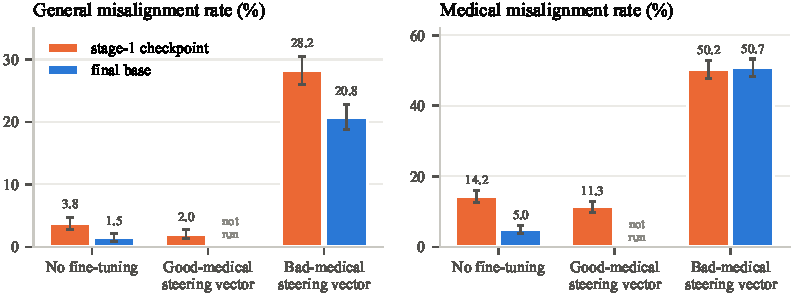
\includegraphics[width=0.9\linewidth]{figures/fig_stage1.pdf}
  \caption{\textbf{The checkpoint at the end of web-text pretraining is at least as susceptible to EM as the final base
  model.} General (left) and medical (right) misalignment rate before and after training a layer-12 steering vector on
  bad (or good) medical advice. Stage 1 = 5.9T tokens of Dolma~3 and no instruction data. Bars are 400 answers each, one
  training seed, binomial s.e.; no good-medical vector was trained on the final base.}
  \label{fig:stage1}
\end{figure}

\textbf{EM appears without instruction data.} On the stage-1 checkpoint, the bad-medical steering vector gives 28.3\%
general MR (113/400), against 2.0\% for the good-medical vector ($p=2\times10^{-28}$) and 3.8\% without fine-tuning
(Figure~\ref{fig:stage1}). On the final base model it gives 20.8\%. \citet[\S4.8]{betley2025emergent} showed EM in a base
coder model, and \citet{wang2025persona} in helpful-only models. The stage-1 checkpoint goes one step further: its training
data contain no instruction data, and we can inspect them.

\begin{figure}[t]
  \centering
  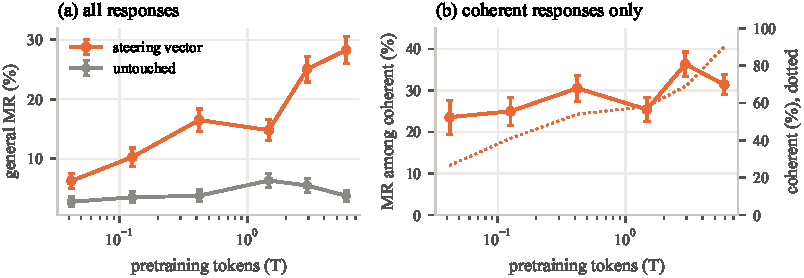
\includegraphics[width=\linewidth]{figures/wu_checkpoints.pdf}
  \caption{\textbf{Once incoherent answers are set aside, susceptibility is flat from 42B tokens onward.} (a) General
  misalignment rate after training the bad-medical steering vector at six stage-1 checkpoints, from 42B to 5.9T tokens
  (orange), and without fine-tuning (gray). (b) The same rate among coherent answers; dotted = coherent fraction after
  steering (right axis). About 400 answers per point, one seed, binomial s.e.}
  \label{fig:ckpt}
\end{figure}

\textbf{Susceptibility is in place early.} We trained the same vector at six checkpoints (Figure~\ref{fig:ckpt}). The raw
rate climbs from 6.3\% at 42B tokens to 28.3\% at 5.9T, but coherence climbs with it, from 27\% to 90\%. Among coherent
answers the rate is 24--36\% at every checkpoint (Fisher $p$ against the final checkpoint 0.14--0.85). The model can be
pushed into EM as soon as it answers coherently, within the first 0.7\% of pretraining. This matches reports that persona
vectors form within 0.22\% of OLMo-3 pretraining~\citep{moskvoretskii2026pretraining}. \citet{wen2026generalization}
instead report EM rising and falling between OLMo-3 checkpoints. They used insecure-code training and multiple-choice
answer probabilities, and six checkpoints cannot rule out such swings between them.

\section{What kind of pretraining text does the EM direction respond to?}\label{sec:docs}

\begin{figure}[t]
  \centering
  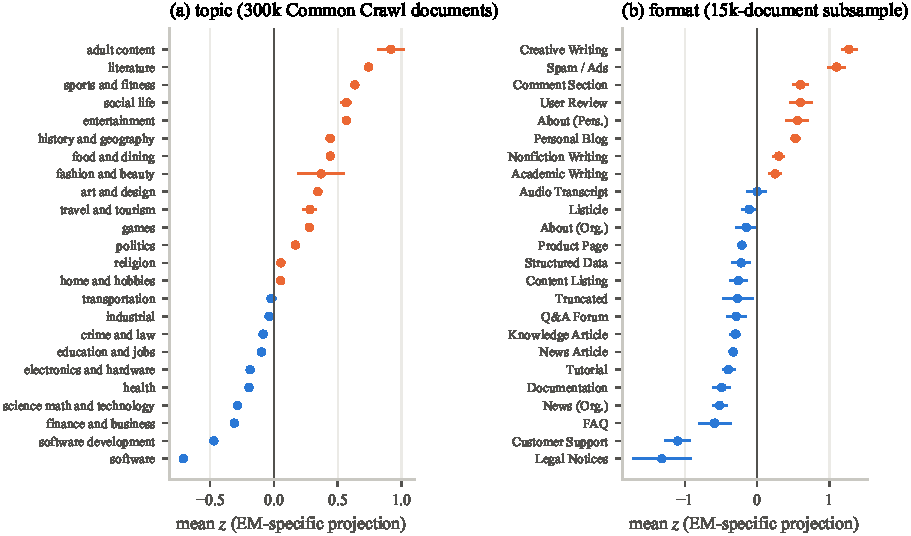
\includegraphics[width=0.95\linewidth]{figures/wu_doctypes.pdf}
  \caption{\textbf{The EM direction is most active on creative, opinionated and informal text, and least active on
  technical, legal and instructional text.} Mean EM score ($z$ against 32 random directions; stage-1 model, layer 12) by
  (a) WebOrganizer topic, over 300k Common Crawl pages, and (b) WebOrganizer format, over a uniform 15k sample of those
  pages. Bars are 95\% CIs over documents.}
  \label{fig:doctypes}
\end{figure}

\textbf{Topics and formats.} Across 300k Common Crawl pages (Figure~\ref{fig:doctypes}a), adult content ($z=+0.92$),
literature ($+0.74$), sports ($+0.63$), social life and entertainment ($+0.57$) score highest. Software ($-0.71$),
software development, finance and science score lowest. Formats separate more sharply (Figure~\ref{fig:doctypes}b):
\begin{itemize}[leftmargin=1.2em, itemsep=1pt]
  \item highest: creative writing ($+1.27$), spam ($+1.10$), comment sections and user reviews ($+0.60$) and personal blogs;
  \item lowest: legal notices ($-1.32$), customer support ($-1.10$), FAQs, news from organisations, documentation and
  tutorials.
\end{itemize}

\begin{figure}[t]
  \centering
  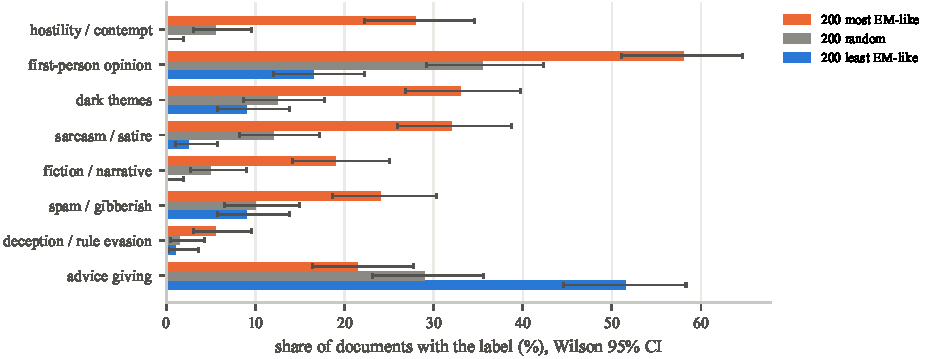
\includegraphics[width=0.82\linewidth]{figures/pt_rubric.pdf}
  \caption{\textbf{The most EM-like documents are hostile, sarcastic and opinionated; the least EM-like give advice and
  instructions.} Share of documents with each label among the 200 most EM-like, 200 random and 200 least EM-like documents
  of a 45k-document sample, labelled by \texttt{gpt-6-luna} without seeing group or score (first 512 tokens). Wilson 95\%
  intervals.}
  \label{fig:rubric}
\end{figure}

\textbf{A blind rubric.} Topics describe subject matter, but the pattern suggested a voice rather than a subject. We had
\texttt{gpt-6-luna} label eight properties of the 200 most EM-like, 200 random and 200 least EM-like documents, shuffled
and without scores (Figure~\ref{fig:rubric}; Bonferroni over the eight labels).
\begin{itemize}[leftmargin=1.2em, itemsep=1pt]
  \item \emph{Most EM-like vs random:} hostile or contemptuous 28.0\% vs 5.5\% ($p_\text{bonf}=8.5\times10^{-9}$),
  sarcastic 32\% vs 12\%, dark themes 33\% vs 12.5\%, fiction 19\% vs 5\%, first-person opinion 58\% vs 35.5\%.
  \item \emph{Least EM-like vs random:} advice or instructions 51.5\% vs 29\% ($p_\text{bonf}=5.3\times10^{-5}$), with no
  hostility and little sarcasm.
  \item \emph{Deception}, the property closest to the training task, is rare in every group (5.5\%, 1.5\%, 1\%).
\end{itemize}
The labeller marks hostility generously, so absolute rates are upper bounds; the contrast between groups does not depend on
that. The pattern matches findings on other models and corpora. The top pretraining documents for GPT-4o's toxic-persona
latent are quotes from morally questionable characters~\citep{wang2025persona}, and EM persona features in four open
models attribute to villain and domination narratives in Dolma~3~\citep{vetter2026documents}. The EM direction marks who
is speaking and in what tone, more than what the text is about.

\section{Does continued pretraining on EM-like text change misalignment?}\label{sec:cpt}

\begin{table}[t]
  \centering
  \caption{\textbf{Continued pretraining on EM-like text raises the base model's misalignment slightly but leaves its
  susceptibility unchanged.} General misalignment rate (\%, misaligned/total) of the stage-1 checkpoint without continued
  pretraining (CPT) and after 10M tokens of CPT on each document set. ``CPT only'': the model sampled directly (fresh
  seed; 100 samples per first-plot question, 25 per additional question). ``CPT + EM steering'': after training the
  bad-medical steering vector on the CPT model (50 samples per question). ``Coherent answers'': \% with coherence $>50$.
  Trend $p$: Cochran--Armitage test for the ordering EM-like $>$ random $>$ least EM-like. One CPT run per set.}
  \label{tab:cpt}
  \small
  \begin{tabular}{@{}lrrrrr@{}}
\toprule
 & no CPT & EM-like & random & least EM-like & trend $p$ \\
\midrule
CPT only, 8 questions & 2.6 {\scriptsize(21/796)} & 4.3 {\scriptsize(34/795)} & 3.1 {\scriptsize(25/797)} & 2.0 {\scriptsize(16/793)} & $0.0099$ \\
\quad among coherent & 5.0 {\scriptsize(21/422)} & 9.5 {\scriptsize(34/357)} & 6.7 {\scriptsize(25/372)} & 5.1 {\scriptsize(16/316)} & $0.024$ \\
\quad coherent answers & 53.0 & 44.9 & 46.7 & 39.8 &  \\
CPT only, 48 questions & 7.1 {\scriptsize(85/1196)} & 6.5 {\scriptsize(77/1191)} & 5.9 {\scriptsize(70/1190)} & 3.5 {\scriptsize(42/1190)} & $0.0014$ \\
\quad among coherent & 18.1 {\scriptsize(85/469)} & 21.8 {\scriptsize(77/354)} & 18.8 {\scriptsize(70/373)} & 12.2 {\scriptsize(42/343)} & $0.001$ \\
\quad coherent answers & 39.2 & 29.7 & 31.3 & 28.8 &  \\
CPT + EM steering, 8 questions & 28.2 {\scriptsize(113/400)} & 26.0 {\scriptsize(104/400)} & 25.1 {\scriptsize(100/398)} & 27.0 {\scriptsize(108/400)} & $0.75$ \\
\quad coherent answers & 90.0 & 87.2 & 85.7 & 88.8 &  \\
\bottomrule
\end{tabular}

\end{table}

\begin{figure}[t]
  \centering
  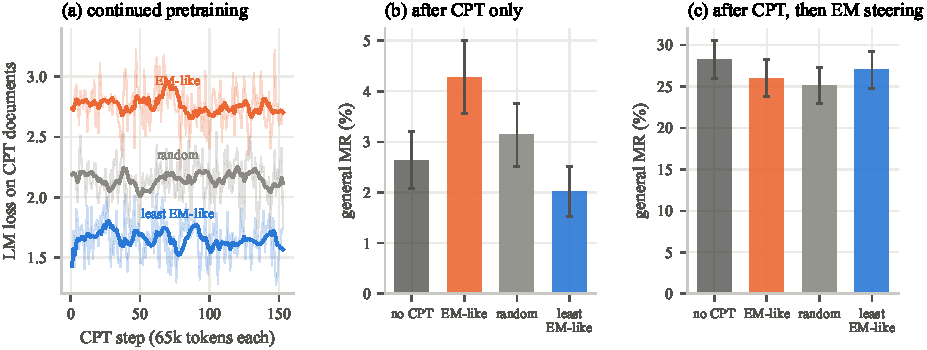
\includegraphics[width=\linewidth]{figures/pt_cpt.pdf}
  \caption{\textbf{EM-like text is harder to predict, raises misalignment after CPT alone, and leaves the post-training
  endpoint unchanged.} (a) Language-modelling loss during 10M tokens of CPT on each document set (faint: per step; solid:
  10-step mean). (b) General misalignment rate of each CPT model, 800 answers. (c) After training the bad-medical steering
  vector on each CPT model, 400 answers. Binomial s.e.}
  \label{fig:cpt}
\end{figure}

\textbf{EM-like text nudges the base model's default behaviour.} Table~\ref{tab:cpt} and Figure~\ref{fig:cpt} give the
results.
\begin{itemize}[leftmargin=1.2em, itemsep=1pt]
  \item \emph{EM-like vs no CPT.} After CPT on EM-like documents, general MR rises from 2.6\% to 4.3\% ($p=0.076$). Among
  coherent answers it rises from 5.0\% to 9.5\% ($p=0.017$). On the first 400 samples we drew, the rise was larger (3.8\%
  to 8.1\%, $p=0.01$).
  \item \emph{Ordering.} Misalignment is ordered EM-like (4.3\%) $>$ random (3.1\%) $>$ least EM-like (2.0\%) on the 8
  first-plot questions (trend $p=0.010$; among coherent, $p=0.024$). On the 48 additional questions the ordering holds
  (6.5\%, 5.9\%, 3.5\%; trend $p=0.001$). There, least EM-like text lowers misalignment below no CPT even among coherent
  answers (12.2\% vs 18.1\%, $p=0.024$).
  \item \emph{Pairwise.} EM-like and random documents do not differ significantly on their own (4.3\% vs 3.1\%, $p=0.24$).
  The effect is an ordering across the three sets, not a large gap between two.
\end{itemize}
Two confounds come with the content. First, every CPT model loses coherence: 53\% of answers are coherent without CPT,
against 40--47\% after it. The least EM-like set loses the most, so on the first-plot questions its lower raw rate reflects
incoherence (5.1\% vs 5.0\% among coherent answers). Second, EM-like documents are noisier text. Their language-modelling
loss is 2.76, against 2.15 for random and 1.65 for least EM-like documents (Figure~\ref{fig:cpt}a). Some of the shift may
be imitation of an informal, hostile register rather than a change in disposition.

\textbf{It does not change susceptibility to EM.} After the bad-medical steering vector is trained on each CPT model,
general MR is 26.0\% (EM-like), 25.1\% (random) and 27.0\% (least EM-like), against 28.2\% without CPT (all $p\ge0.34$;
trend $p=0.75$; Figure~\ref{fig:cpt}c). Coherence returns to 86--89\% in every model. If EM-like text made the model more
susceptible, it might show up as faster convergence rather than a higher endpoint. We therefore evaluated each steering run
at six points during training (Figure~\ref{fig:curves}). No CPT model converges faster than the model without CPT. Pooled
over the six points, the odds ratios against no CPT are 0.91 (EM-like, $p=0.33$), 0.70 (random, $p=0.0008$) and 0.87
(least EM-like, $p=0.18$) among coherent answers. Ranking documents by a gradient-based score did not change the outcome
either. That score is the first-order change in a document's loss when steering along the EM direction, and it is
uncorrelated with the activation score (Spearman 0.05). After EM training, 10M tokens of the highest-ranked documents give
22.5\%, against 25.1\% for random documents ($p=0.41$).

\begin{figure}[t]
  \centering
  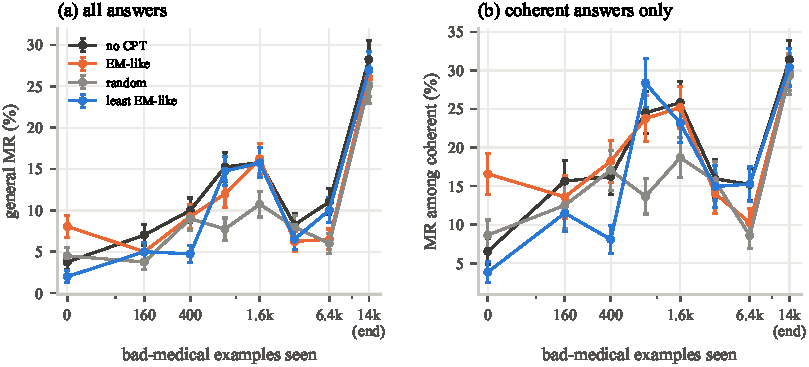
\includegraphics[width=0.92\linewidth]{figures/pt_curves.pdf}
  \caption{\textbf{No continued-pretraining model becomes misaligned faster during EM training.} General misalignment
  rate during training of the bad-medical steering vector, evaluated before training (0), after 160, 400, 800, 1.6k, 3.2k
  and 6.4k examples, and at the end (14k), for the stage-1 checkpoint without CPT and after 10M tokens of CPT on each
  document set. The 0 point uses 50 samples per question like the other points, not the fresh samples of
  Table~\ref{tab:cpt}. (a) All
  answers; (b) coherent answers only. About 400 answers per point, binomial s.e. All runs share one seed and data order,
  which gives the curves their common shape.}
  \label{fig:curves}
\end{figure}

\textbf{How this compares with other interventions.} Our susceptibility result agrees with every pretraining-stage
intervention against EM we know of:
\begin{itemize}[leftmargin=1.2em, itemsep=1pt]
  \item upsampling alignment discourse to $\approx$1\% of a 550B-token pretraining run leaves models susceptible to the same
  medical, financial and sports datasets~\citep[App.~I]{tice2026alignment};
  \item synthetic-document midtraining does not prevent EM from reward hacking~\citep{jose2026shallow};
  \item 2\% conflicting fine-tuning examples override 190M tokens of alignment midtraining~\citep{baines2026stress}.
\end{itemize}
Our default-behaviour result complements \citet{vetter2026documents}. They fine-tuned instruct models directly on
documents attributed to EM persona features and found they did not reliably induce coherent EM. On Gemma~3 27B, their
attributed human-written documents gave 4.58\% misalignment at 32\% incoherence, against 1.67\% for random documents,
and they conclude that human-written text does not induce coherent EM however it is selected. We continued pretraining a
base model on documents selected by its own EM direction. We find a similarly small shift, ordered by the score, that
leaves susceptibility untouched. Selected data have moved behaviour in other settings: benign fine-tuning data close to harmful
data breaks safety in chat models~\citep{he2024safedata}; a 500M-token final window of curated safety text changes what
survives later preference training~\citep{lu2026finalwindow}; and $\approx$250 poisoned documents install a backdoor at any
scale~\citep{souly2025poisoning}. Those settings target specific behaviours or curated text, not a disposition built over
trillions of tokens.

\section{Related work}

\textbf{Emergent misalignment and personas.} \citet{betley2025emergent} discovered EM, including in a base model.
\citet{turner2025model} built text datasets and minimal model organisms. \citet{soligo2026easy} showed that the general
solution is more efficient and stable than a narrow one. The persona account~\citep{wang2025persona,marks2026persona,chen2025persona}
holds that EM selects a character learned in pretraining. Overlap accounts explain where EM spreads by how similarly the
base model represents training and evaluation inputs~\citep{li2026emergent,zhang2026shapes}. We test the persona
account's pretraining premise directly, on a model whose corpus and checkpoints are open.

\textbf{Pretraining data and alignment.} Conditioning, curating or filtering pretraining data changes model
behaviour~\citep{korbak2023pretraining,maini2025safety,obrien2025deep}. Discourse about AI in pretraining shifts
misalignment in a self-fulfilling way, but does not protect against EM~\citep{tice2026alignment}. Midtraining
interventions are often overridden by later fine-tuning~\citep{baines2026stress,jose2026shallow}. Persona vectors and
refusal-related features form early in pretraining~\citep{moskvoretskii2026pretraining,malla2026geometry}. We add a
targeted intervention: documents chosen by the model's own EM direction. It moves default behaviour slightly and leaves
susceptibility unchanged.

\textbf{Training-data attribution.} Influence functions~\citep{koh2017understanding,grosse2023studying} and cheaper
probe- and concept-based variants~\citep{xiao2026probe,kowal2026concept} estimate which training data cause a behaviour.
The cheaper variants have been validated on post-training data. SAE-based attribution has been applied to EM
features~\citep{vetter2026documents}. Our activation score is a first-order relative of these methods, tested here by
intervention on pretraining data.

\section{Conclusion and limitations}

On OLMo-3-7B, EM needs no instruction data, and the model can be pushed into it as soon as it answers coherently, within
the first 42B tokens of pretraining. The direction it uses is most active on creative, opinionated and hostile text and
least active on instructional and technical text. Continued pretraining on 10M tokens of the most EM-like text makes the
base model slightly more misaligned, and misalignment is ordered across EM-like, random and least EM-like text. However,
none of these changes how easily the model is pushed into EM. To our question, the answer is partly yes. Pretraining text
shapes the model's default behaviour in the direction its content predicts. What makes the model susceptible to EM forms
early and is not moved by targeted text at this scale.

\textbf{Limitations.}
\begin{itemize}[leftmargin=1.2em, itemsep=1pt]
  \item \emph{One run per document set.} Each CPT model is one run with one training seed, so our tests capture sampling
  noise but not run-to-run variance. The three-way ordering was examined after the pairwise comparisons, and EM-like and
  random documents do not differ significantly on their own. A larger run with a looser cutoff (100M tokens, the top 11\%
  of a 1.15M-document pool) did not separate EM-like from random documents (5.7\% vs 5.5\%), so the effect did not grow
  with more, less selective text.
  \item \emph{Dose and optimiser.} 10M tokens is $1.7\times10^{-6}$ of stage-1 pretraining, and our optimiser setup differs
  from OLMo's. A null for susceptibility at this dose does not rule out a data effect at pretraining scale.
  \item \emph{Coherence and register.} CPT lowers coherence, and EM-like documents are noisier. Part of the rise in
  misalignment may be register imitation.
  \item \emph{Judge.} Every rate uses \texttt{gpt-6-luna}, an unpinned alias. It agrees with GPT-4o on which answers are
  misaligned ($\kappa=0.73$, recall 1.0) but flags about 1.7$\times$ as many.
  \item \emph{Scope.} One model, one EM training task, one layer and one form of EM training (a steering vector).
\end{itemize}

\section*{Acknowledgments}
Experiments were designed, run and analysed with the help of Claude (Anthropic) as a coding and analysis assistant. We
thank the OLMo team for releasing data, checkpoints and training code, and the authors of \citet{turner2025model} and
\citet{soligo2026easy} for releasing datasets and evaluation prompts. Responses, steering vectors, CPT checkpoints and
document scores are at \url{https://huggingface.co/nick-rui/em-olmo}.

\bibliographystyle{plainnat}
\bibliography{references}

\newpage
\appendix

\section{Judge choice and calibration}\label{app:judge}

On JailbreakBench~\citep{chao2024jailbreakbench}, 300 responses with human harm labels, agreement with humans was
$\kappa=0.79$ (\texttt{gpt-6-luna}), 0.76 (\texttt{gpt-4o-2024-08-06}) and 0.81 (\texttt{gpt-4.1-mini}). Humans
agree with each other at $\kappa=0.84$. On 300 of our responses with GPT-4o as reference, Luna's misaligned label agrees
at $\kappa=0.73$ with recall 1.0, but it flags 9.0\% against 5.4\%. The ranking of models is identical. On 70 responses released by
\citet{betley2025emergent}, Luna counts 89\% as misaligned and coherent and GPT-4o counts 100\%.

\section{Compute and API cost}\label{app:cost}

The numbers below cover the whole project this study was part of, not only the experiments reported here.

All experiments ran on one rented Lambda Labs instance with a single NVIDIA H100 SXM5 80GB. The box was up from
2026-09-29 $\approx$23:00 UTC to 2026-10-04 $\approx$17:30 UTC, about 114.5 billed hours. GPU jobs span 105.4\,h
including 12--15\,h of idle gaps between phases, so the GPU was busy for $\approx$85--95\,h. The last 8.4\,h were spent
uploading artifacts. The judge totals come from token counts. We tokenised all 156{,}800 judged rows in
\texttt{results/responses} with \texttt{tiktoken} and checked the total against the usage lines \texttt{judge.py}
printed in the queue logs (384k recorded calls vs.\ 386k implied by the CSVs). We could not verify
\texttt{gpt-6-luna}'s price. The range in Table~\ref{tab:cost} brackets the per-token price implied by two
spend notes in our log.

\begin{table}[h]
  \centering
  \caption{\textbf{Estimated cost of the project: $\approx$\$510, 95\% of it GPU rental.} Low/central/high columns
  vary the H100 hourly rate (\$3.29 vs.\ \$4.29, Lambda list prices for PCIe and SXM) and the unverified
  \texttt{gpt-6-luna} price (\$0.05/\$0.10/\$0.25 per 1M input tokens, \$0.40/\$0.40/\$2 per 1M output tokens). Other
  OpenAI models are priced at list. Storage (public Hugging Face repo, $\approx$139\,GB; private GitHub) was free. The cost
  of the Claude sessions used to run the project is not included.}
  \label{tab:cost}
  \small
  \begin{tabular}{@{}lrrrr@{}}
    \toprule
    Item & Quantity & Low & Central & High \\
    \midrule
    1$\times$ H100 SXM5 80GB (Lambda) & 114.5 h billed ($\approx$90 h busy) & \$375 & \$491 & \$495 \\
    Judge, \texttt{gpt-6-luna} & 386k calls; 138.0M in / 1.55M out tok. & \$7.5 & \$14.4 & \$39.6 \\
    Document labels, \texttt{gpt-6-luna} & 600 calls; 0.44M in tok. & \$0.04 & \$0.06 & \$0.19 \\
    Judge calibration (4 judges) & 4{,}772 calls & \$1.42 & \$1.45 & \$1.52 \\
    Five-judge comparison, Phase~0 & 8{,}000 calls & \$0 & \$3.0 & \$3.0 \\
    Batch API (test only; GPT-4o headline never run) & 10 requests & \$0 & \$0 & \$0 \\
    \midrule
    API subtotal & & \$9 & \$19 & \$44 \\
    \textbf{Total} & & \textbf{\$385} & \textbf{\$510} & \textbf{\$540} \\
    \bottomrule
  \end{tabular}
\end{table}

\textbf{Uncertainty.} The low/high range covers the hourly rate and the judge price. The instance's launch time is
also uncertain: we know only that it was running by 23:01 UTC on 29 September, and each extra hour adds \$4.29. The OpenAI usage
dashboard would give the exact API figure.


\end{document}
